\chapter{The Detector}

\section{The Layout of CERN}

The Large Hadron Collider (LHC), operated by the CERN collaboration, is a 27-kilometer long proton-proton circular collider located underneath the border area of France and Switzerland, outside the city of Geneva (Figure~\ref{fig:LHC}). The LHC consists of a circular ring, around which two proton beams are accelerated in opposite directions under the guidance of powerful superconducting magnets. These proton beams are allowed to intersect at four beam-crossing points around the ring, where they are smashed head-on at a center-of-mass energy of 13 TeV. There are seven particle detectors stationed around the crossing points to observe the resulting collisions. One of these detectors, ATLAS, is the source of data used in this thesis.

\begin{figure}[htbp]
    \centering
    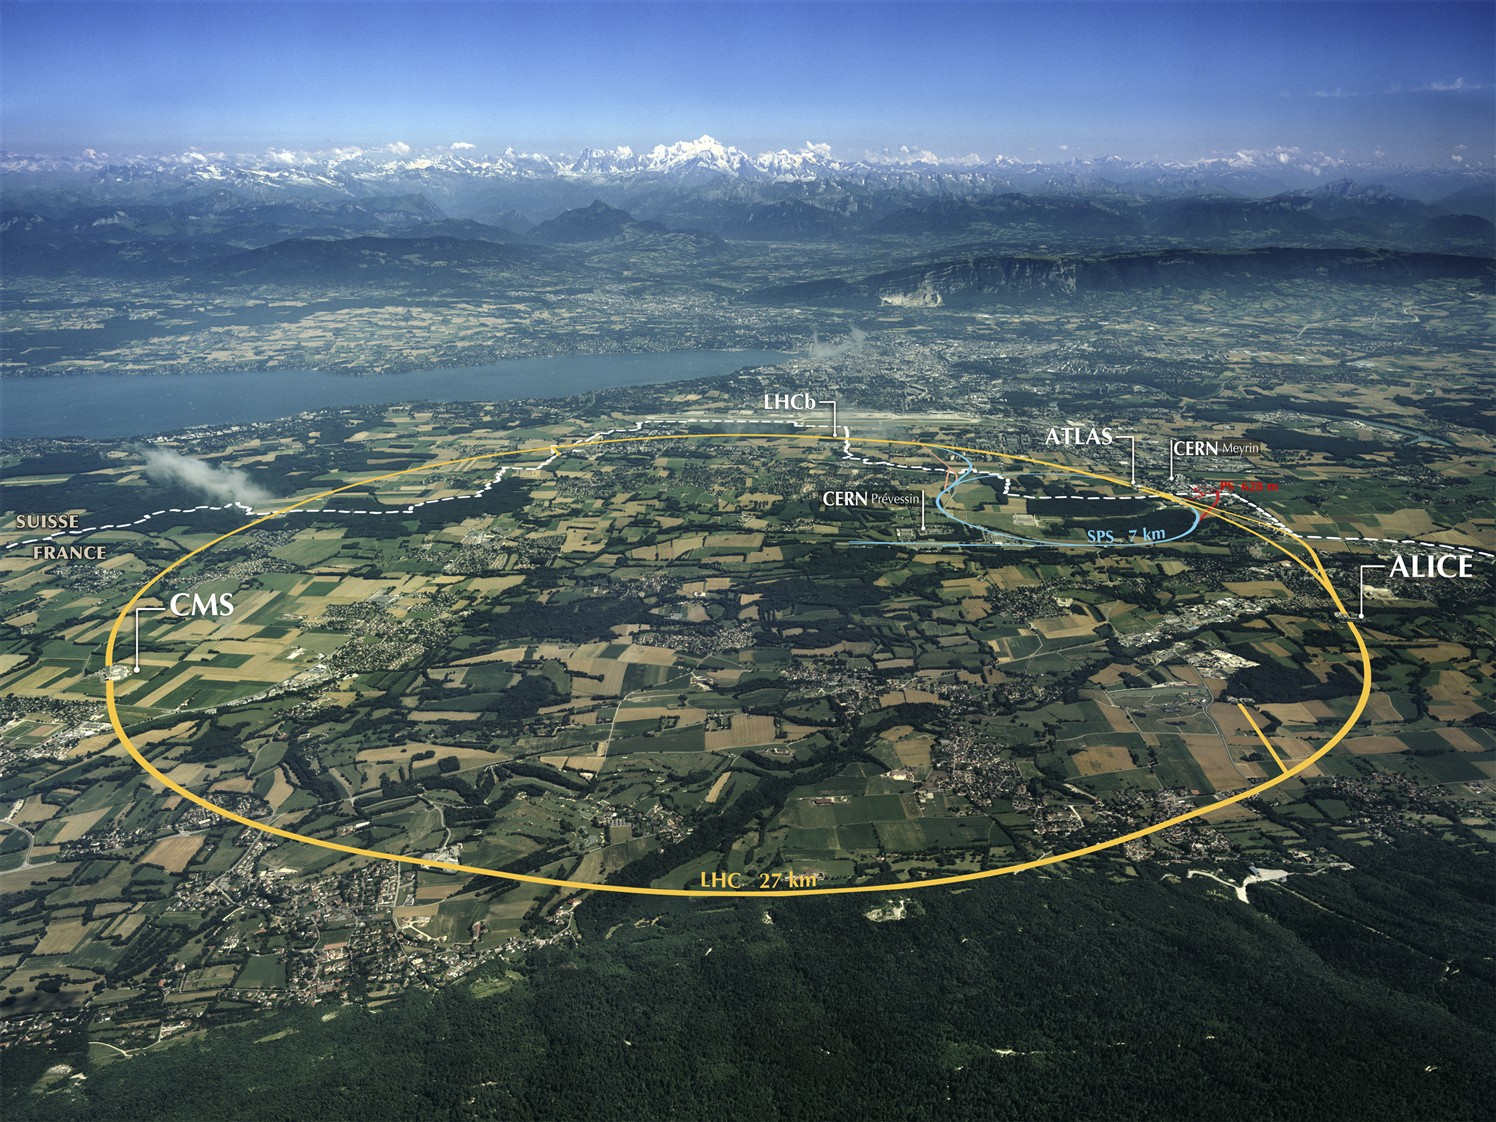
\includegraphics[width=\linewidth]{Images/ATLAS/LHC.jpg}
    \caption{An overhead view of the LHC. Image taken from~\cite{LHC}.}
    \label{fig:LHC}
\end{figure}

\section{An Anatomy of ATLAS}

The ATLAS detector (Figure~\ref{fig:ATLAS}), built around one of the LHC beam crossing points, acts as a eight-story-tall recording device for capturing and digitizing the results of collisions. The detector contains multiple types of detection technology, each specialized to perform a specific type of measurement~\cite{ATLAS_detector}.

\begin{figure}[htbp]
    \centering
    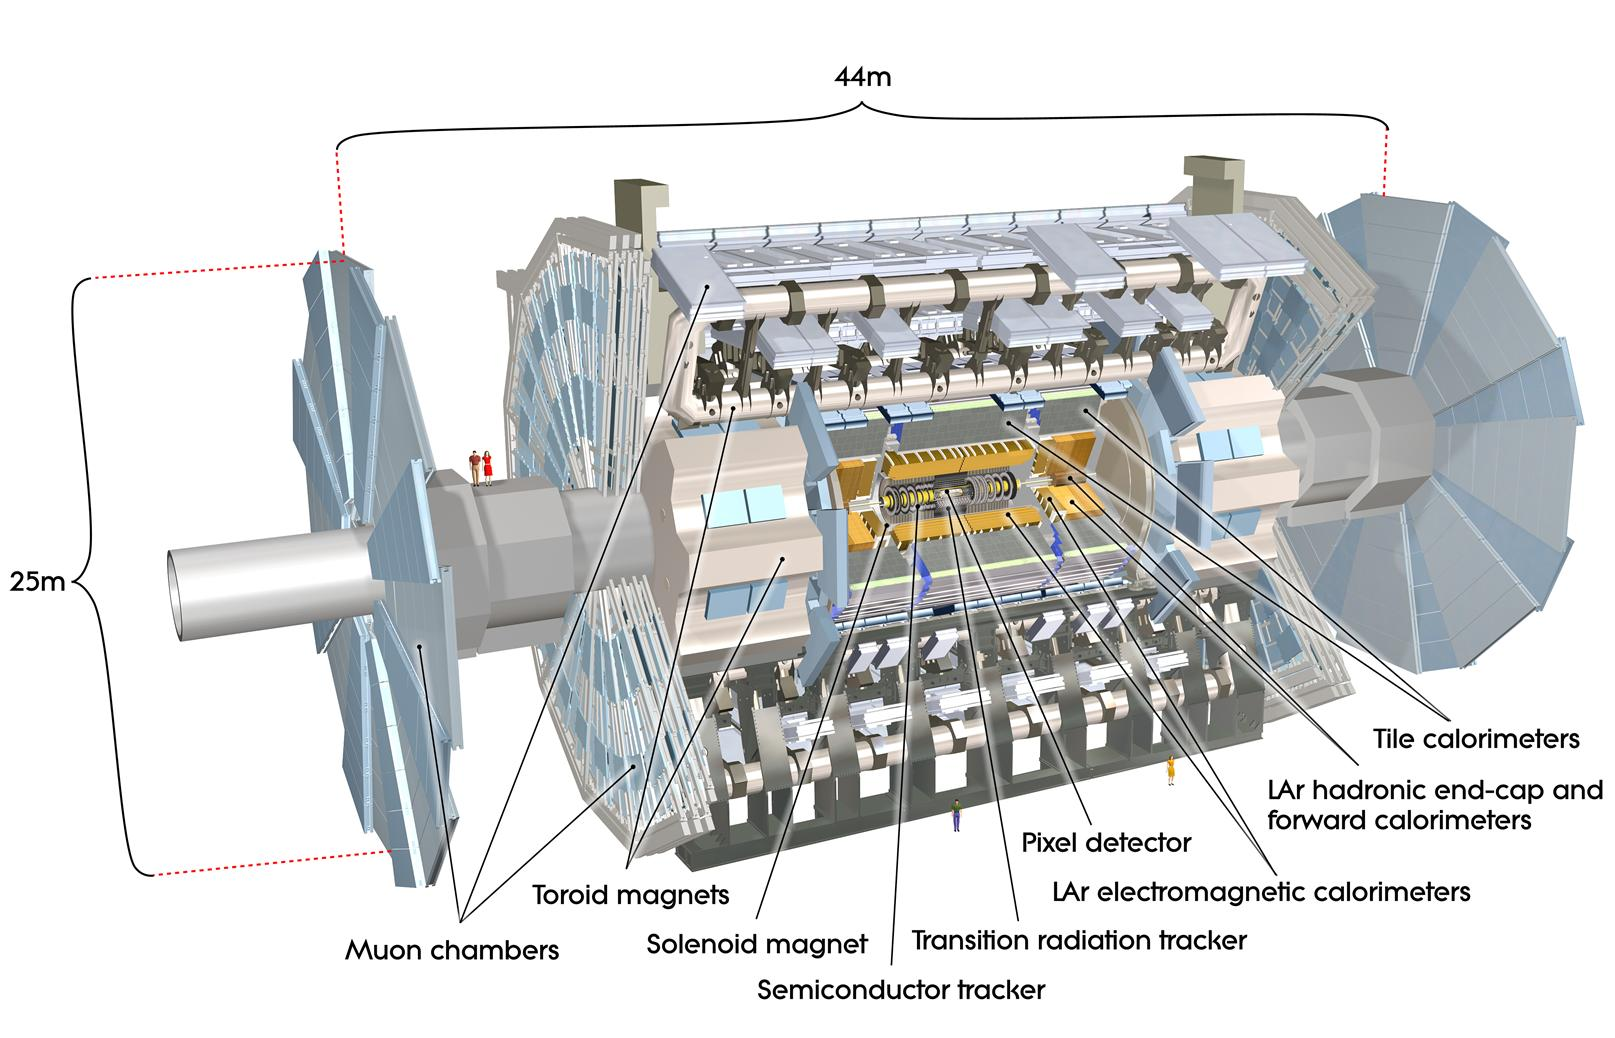
\includegraphics[width=\linewidth]{Images/ATLAS/ATLAS.jpg}
    \caption{A labeled diagram of the ATLAS detector. Figure from~\cite{ATLAS_detector}.}
    \label{fig:ATLAS}
\end{figure}

The backbone of ATLAS consists of a beam pipe surrounded by a solenoid magnet. The protons traverse through the beam pipe and collide, and the resulting particles are curved as they propagate in the plane perpendicular to the beam. Surrounding the beam and the interaction point, we have the inner detector, the calorimeters, and the muon spectrometers (though they have been labelled a bit differently in Figure~\ref{fig:ATLAS}). A partial cross-section view of the detector is shown in Figure~\ref{fig:ATLAS_cross_section}.

\begin{figure}[htbp]
    \centering
    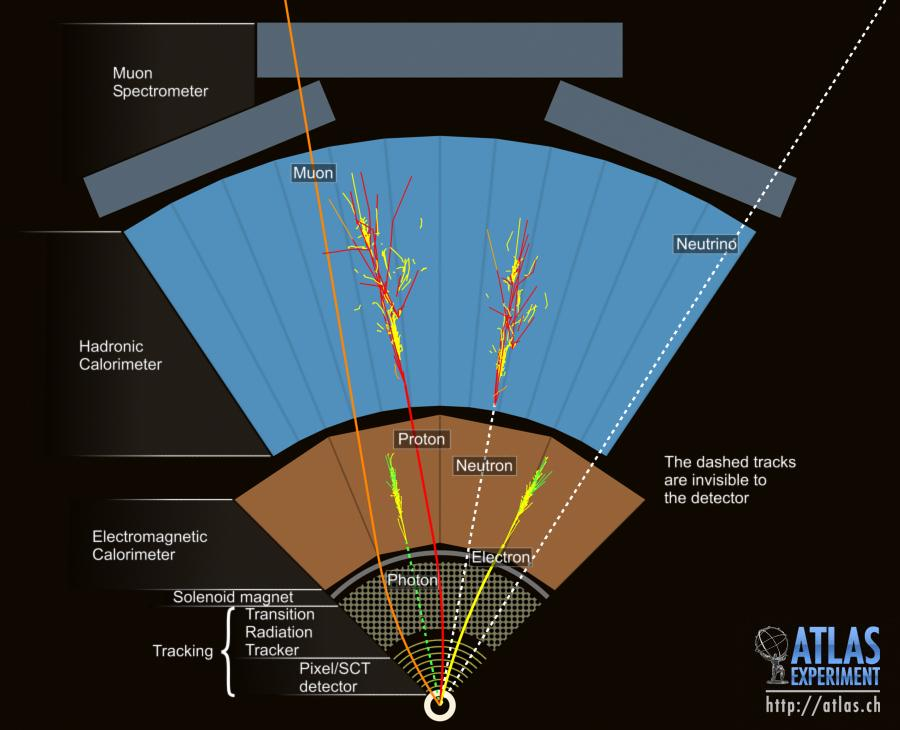
\includegraphics[width=\linewidth]{Images/ATLAS/ATLAS_cross_section.jpg}
    \caption{A cross section of the ATLAS detector. Figure from~\cite{ATLAS_cross_section}.}
    \label{fig:ATLAS_cross_section}
\end{figure}

The inner detector is composed of the silicon pixel and strip detectors and the transition radiation tracker (TRT)~\cite{ATLAS_inner_detector_TDR}. This portion of the detector is used to reconstruct tracks for charged particles, with which we determine their flight paths, momenta, and points of origin. The pixel and strip (SCT) detectors are both silicon-based, and operate via the generation of a depletion region in the material. When charged particles travel through the silicon, they generate electron-hole pairs, which propagate under an applied voltage and are captured via readout chips. The pixel detectors compose the innermost layers, and are segmented finely in both $\eta$ and $\phi$, so as to capture more precise spatial information. The strip detectors are outside the pixel layers, and are segmented only in $\phi$. TRT layers are outside the silicon layers, and consist of Kapton-carbon tubes surrounding tungsten wires. The wires and tubes are kept at a voltage potential, and the space in between is filled with a majority-xenon gas mixture. Once again, passing charged particles ionize the bulk material (in this case the gas), and the resulting electron-hole pairs are captured via the voltage gradient and read out by specialized electronics.

After the inner trackers and the solenoid magnet, we have the calorimeters~\cite{calorimeters_intro}. First we have the electron calorimeter (ECAL), which captures and records the energies of electrons and photons through EM interactions. The hadronic calorimeter (HCAL) is after that, and being composed of heavy elements, it forces hadronic particles to deposit their energies through strong interactions. Each of these calorimeters causes particle showering to occur, during which many charged particles are produced. These particles can then either produce visible photons via scintillation, or produce electron-hole pairs via ionization. The calorimeters are composed of the cylindrical sections concentric to the beam pipe, in what is called the barrel, and the disks on the sides perpendicular to the beam pipe, in what are called the end caps. The ECAL in ATLAS uses liquid argon sampling calorimeters, while the HCAL uses lead and plastic scintillators in the barrel and liquid argon in the endcaps. The ECAL encloses its liquid argon in accordian-like cells, relying on ionization and charge capture, while the HCAL uses alternating planes of lead and plastic, with the lead inducing showering and the plastic capturing the information via scintillation. The deposited energy is determined linearly via the collected signal. The resulting calorimeter energy resolution goes as the following, where $\sigma$ is the resolution, $a$ is statistical due to the number of charged particles produced, $b$ is due to noise and pileup from soft collisions (surrounding collisions, other than the one we're interested in), and $c$ is due to calorimeter errors:

\begin{align}
    \frac{\sigma}{E} &= \frac{a}{\sqrt{E}} \oplus \frac{b}{E} \oplus c
\end{align}

Finally, the detector is ringed by muon spectrometers, which detect the penetrating muons that pass through the rest of the detector~\cite{ATLAS_TDR}. The spectrometers are composed of a barrel section and end caps, and are in charge of precisely measuring the curvature of muons via mechanisms such as drift tubes.

As seen in Figure~\ref{fig:ATLAS_cross_section}, photons and electrons are typically stopped in the ECAL, and protons and neutrons are typically stopped in the HCAL. Charged particles, including electrons, protons, and muons, leave hits in the inner detector. Muons go all the way through the muon detector. Finally, neutrinos pass through ATLAS undetected, and their effects are seen in missing transverse momentum when the transverse momenta of all other decay products in the reaction are summed up. Once all the hits in a single collision are recorded, the data is then passed to triggering and reconstruction algorithms to determine what objects were in the event, and whether or not to store the data.

\section{Upgrades}

The LHC currently produces about 40 collisions per beam-crossing at 13 TeV center-of-mass energy, but with the proposed high-luminosity LHC (HL-LHC) upgrade~\cite{HL_LHC}, there are plans to increase these numbers to 140 collisions per beam-crossing at 14 TeV by 2026, amounting to a total of 250 $fb^{-1}$ of data per year, with ultimate plans to increase to 200 collisions per beam-crossing. During the HL-LHC upgrade, ATLAS similarly plans to upgrade its detection capabilities via the ATLAS Phase-II upgrade~\cite{ATLAS_phaseII_TDR}, focusing on items such as replacing the inner detector with an all-silicon-based inner tracker (ITk), improving data acquisition, and increasing the granularity of calorimeters.

The higher data rates and improved calorimeters provide an incentive to develop and implement the machine-vision based particle identification projects described later in this thesis, and also prompted the lepton isolation machine-learning project which will be described later. Furthermore, in the interest of improving upcoming SUSY searches, I have aided in the development of several other components in the ATLAS detector, including both hardware and firmware upgrades for the inner detector, and vertexing algorithms for event reconstruction. Though these projects are not the focus of this thesis, they will be described in the appendices.